\documentclass[pdf, ]{beamer}
\usepackage[]{hyperref, graphicx, siunitx, lmodern, tikz, booktabs, physics}
\usepackage[mode=buildnew]{standalone}
\usepackage{pdfpc-commands}
\usepackage{intro-commands}
\pgfplotsset{compat=1.16}

\usetheme{Astro}
\graphicspath{ {Images/} }

\sisetup{per-mode=symbol}
\usetikzlibrary{calc, patterns, decorations.markings, decorations.pathmorphing, shapes}

\newcommand{\secimg}{SecMoon.png}
\AtBeginSection[]{
	{
	\setbeamertemplate{footline}{}
	\begin{frame}
		\begin{tikzpicture}[remember picture, overlay]
			\fill[Background] (current page.north west) rectangle (current page.south east);
			\node[opacity=0.4, anchor=south east, inner sep=0pt, outer sep=0pt] at ([xshift=2cm]current page.south east) {\includegraphics[width=18cm]{\secimg}};
			\fill[Foreground, opacity=0.8] ([yshift=2cm]current page.west) rectangle ([yshift=1cm]current page.east);
			\node[font=\LARGE, Background, anchor=west] at ([yshift=1.5cm, xshift=1cm]current page.west) {\insertsectionhead};
			\node[font=\small, Foreground, anchor=south west] at ([yshift=2cm]current page.west) {Upcoming:};
		\end{tikzpicture}
	\end{frame}
	}
}
\setbeamertemplate{title page}{%
  \begin{tikzpicture}[remember picture, overlay]
	%\fill[red] (current page.north west) rectangle (current page.east);
	\begin{scope}
		\clip (current page.north west) rectangle ($(current page.east)-(0,2)$);
		\node[opacity=0.8, anchor=south east] at ([yshift=-7cm, xshift=2cm]current page.north east) {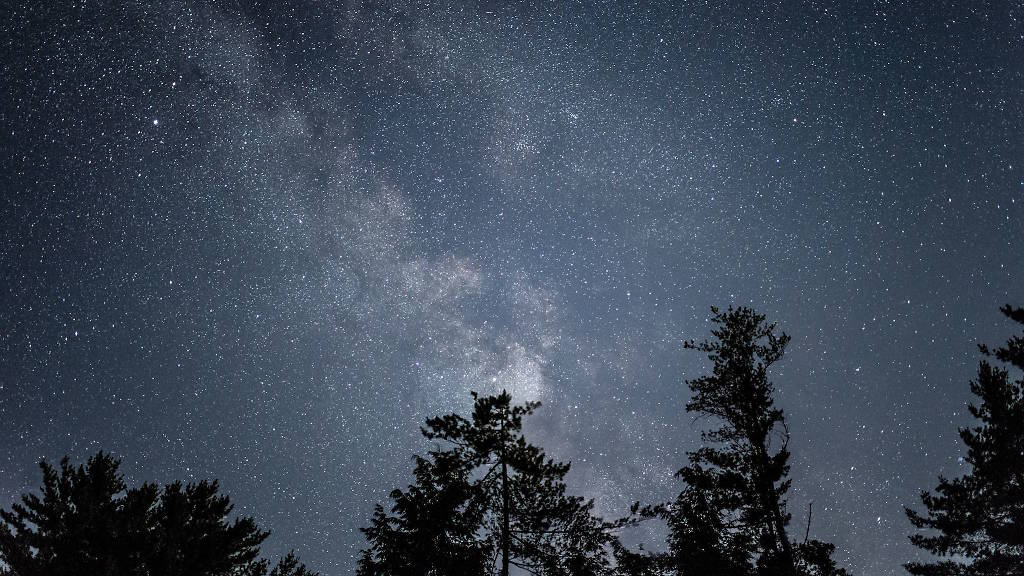
\includegraphics[width=18cm]{CoverSky.png}};

		\node at (3,0) {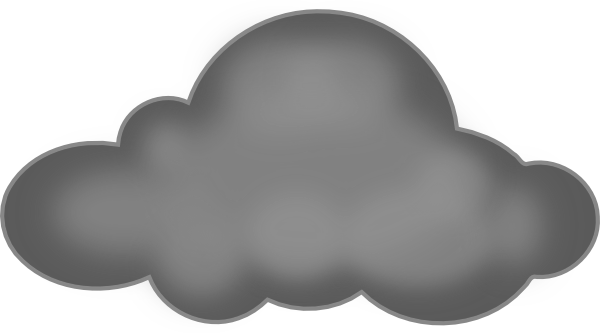
\includegraphics[width=4cm]{Cloud.png}};
		\node at (7,3) {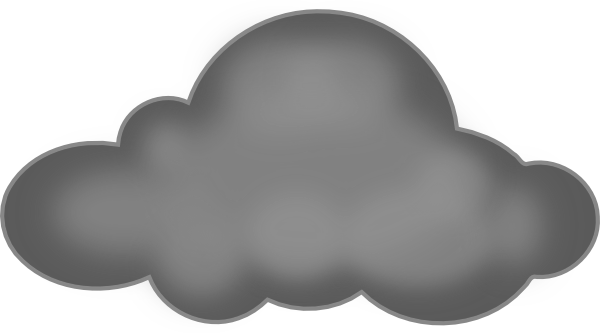
\includegraphics[width=6cm]{Cloud.png}};
		\node at (6,-1) {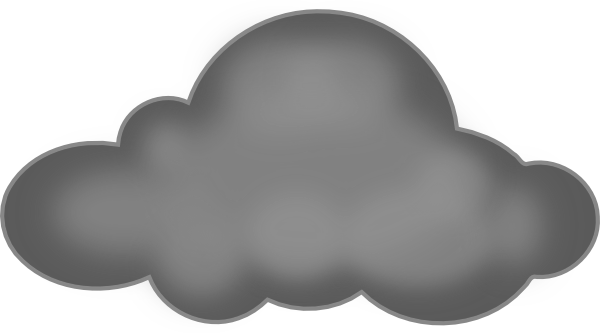
\includegraphics[width=3cm]{Cloud.png}};
		\node at (10,1) {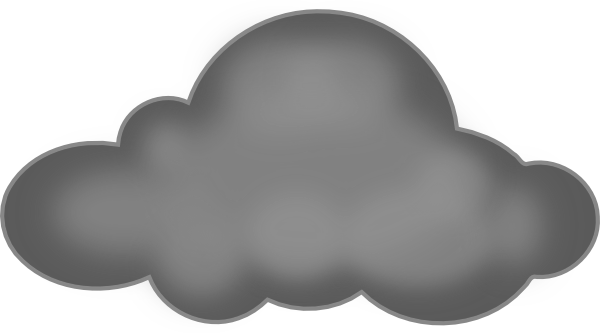
\includegraphics[width=4cm]{Cloud.png}};
		\node at (0,2) {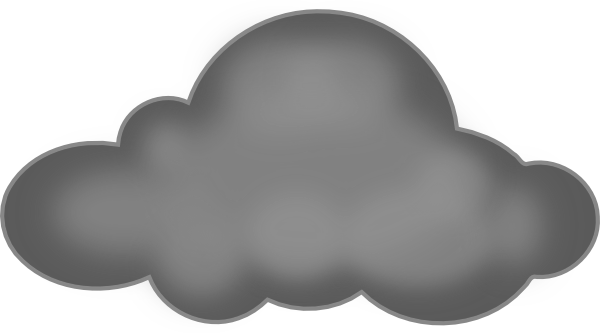
\includegraphics[width=5cm]{Cloud.png}};
		\node[anchor=south east] at ([yshift=-7cm, xshift=2cm]current page.north east) {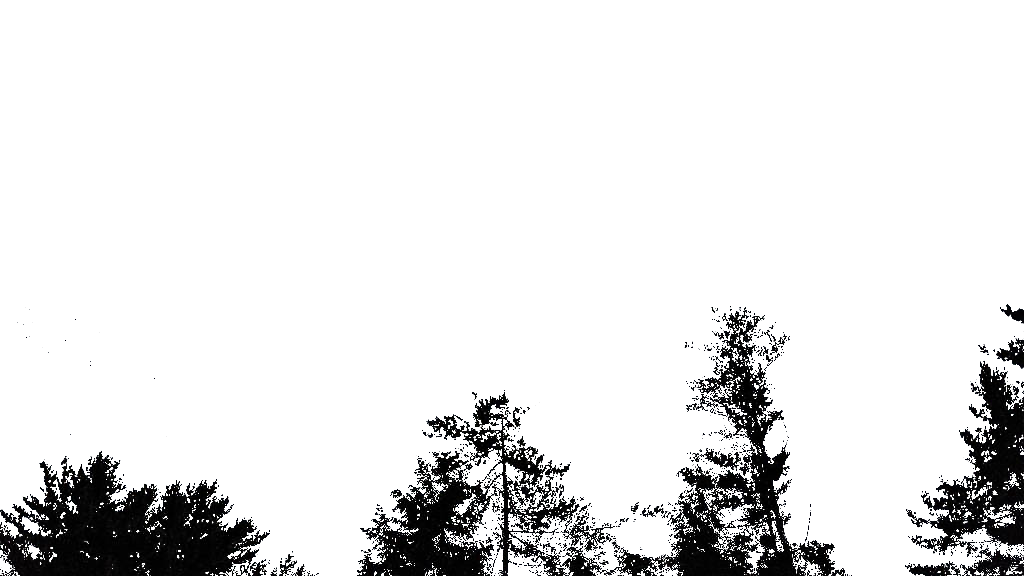
\includegraphics[width=18cm]{CoverSkyForeground.png}};
	\end{scope}
	\node[font={\LARGE}, Orange, anchor=south, inner sep=0pt, outer sep=0pt] at ([yshift=-3cm]current page.center) {\inserttitle};
	%\node[font={\LARGE\scshape}, orange!80, opacity=0.2, anchor=south, inner sep=0pt, outer sep=0pt, yscale=-1, xslant=1.2] at ([yshift=-3cm]current page.center) {\inserttitle};
	%\node[font=\large, gold] at ([yshift=-22mm]current page.center) {\insertsubtitle};
	\node[font=\large, Foreground] (name) at ([yshift=-35mm]current page.center) {\insertauthor};
	\node[gray] at ([yshift=-40mm]current page.center) {\insertinstitute};
	\node[gray] at ([yshift=-44mm]current page.center) {\insertdate};
  \end{tikzpicture}
}

%Preamble
\title{A Guide to Salem's Night Skies}
\author{Jed Rembold}
\institute{Willamette University}
\date{August 3, 2019}

\begin{document}
\renewcommand{\theenumi}{\Alph{enumi}}

{
	\setbeamertemplate{footline}{}
	\maketitle
}

\begin{frame}{Squad Goals}
	\begin{itemize}
		\item To give you a short list of fun, easy things to look at when you find yourself under a night sky
		\item To make sure you know how to find said objects in the sky
			\begin{itemize}
				\item Don't be afraid to use technology to help you either! There are some great apps out there these days.
			\end{itemize}
			
		\item Everything is visible with the naked eye and looks great with just binoculars
		\item A small telescope will really make everything pop but is largely unnecessary
		\item Slides available at \url{https://github.com/jrembold/Presentations} under the SPL Skies of Salem folder for future reference

	\end{itemize}
	
\end{frame}

\begin{frame}{Overview}
	\begin{columns}
		\column{0.5\textwidth}
		\begin{itemize}
			\item The Moon
				\begin{itemize}
					\item Tycho
					\item Copernicus
					\item Sea of Tranquility
				\end{itemize}
			\item Planets
				\begin{itemize}
					\item Jupiter and moons
					\item Saturn
					\item Venus and Mars
				\end{itemize}
		\end{itemize}
		
		\column{0.5\textwidth}
		\begin{itemize}
		\item Deep Sky
			\begin{itemize}
				\item Pleiades
				\item Orion Nebula
				\item Andromeda Galaxy
				\item Hercules Cluster
			\end{itemize}
		\item Other
			\begin{itemize}
				\item Perseid Meteor Shower
				\item ISS and Iridium Flares
			\end{itemize}
		\end{itemize}
	\end{columns}
\end{frame}



\section{The Moon}

\begin{frame}{The Moon}
	\begin{itemize}
		\item Where to find:
			\begin{itemize}
				\item Full: highest in sky around midnight
				\item New: highest in sky at noon
				\item Waxing: up in early evening
				\item Waning: up in early morning
			\end{itemize}
		\item Always see basically the same side of the Moon
			\begin{itemize}
				\item Rotates on axis at same rate it rotates around Earth
			\end{itemize}
		\item Near-side has lots of contrast with darker lowlands and brighter highlands
		\item Looking along the \alert{terminator} where light meets dark, will give the greatest sense of depth and contrast from shadows.
	\end{itemize}
\end{frame}

\begin{frame}{Tycho}
	\begin{columns}
		\column{0.4\textwidth}
		\begin{itemize}
			\item Named after Tycho Brahe
			\item Bright crater in Southern hemisphere
			\item Characterized by many long rays emanating outwards
			\item Fairly young by crater standards
		\end{itemize}
		\column{0.6\textwidth}
		\begin{center}
			\begin{tikzpicture}[scale=0.78]
				\node<1-2> {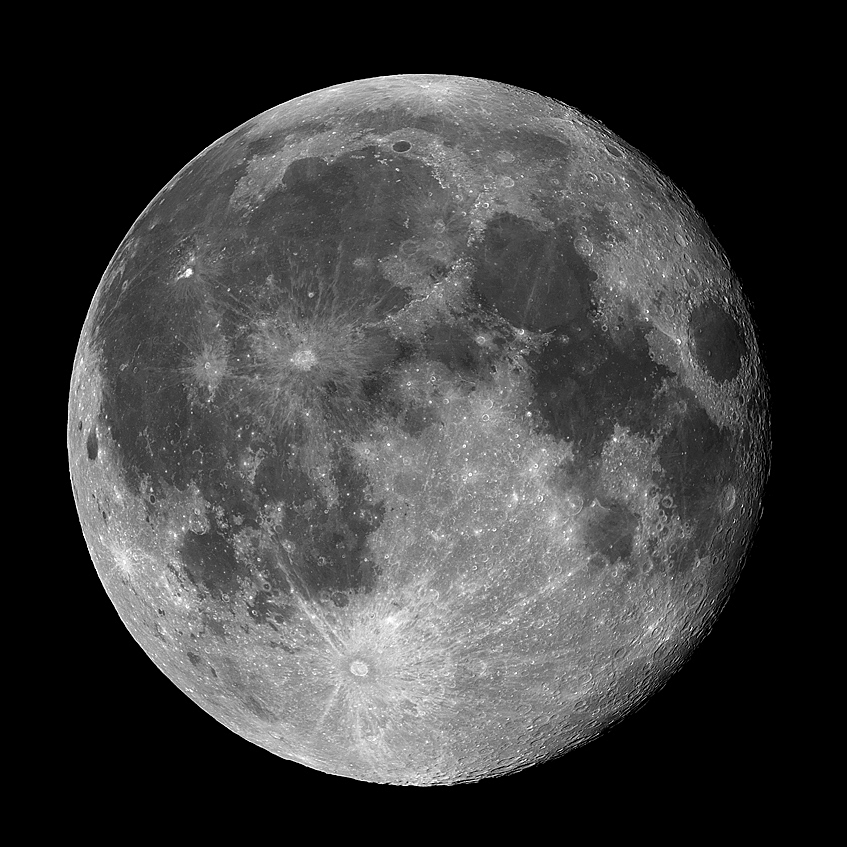
\includegraphics[width=0.8\textwidth]{FullMoon_Barrett.jpg}};
				\draw<2>[very thick, red] (-.5,-1.9) circle (4mm);
				\node<3> {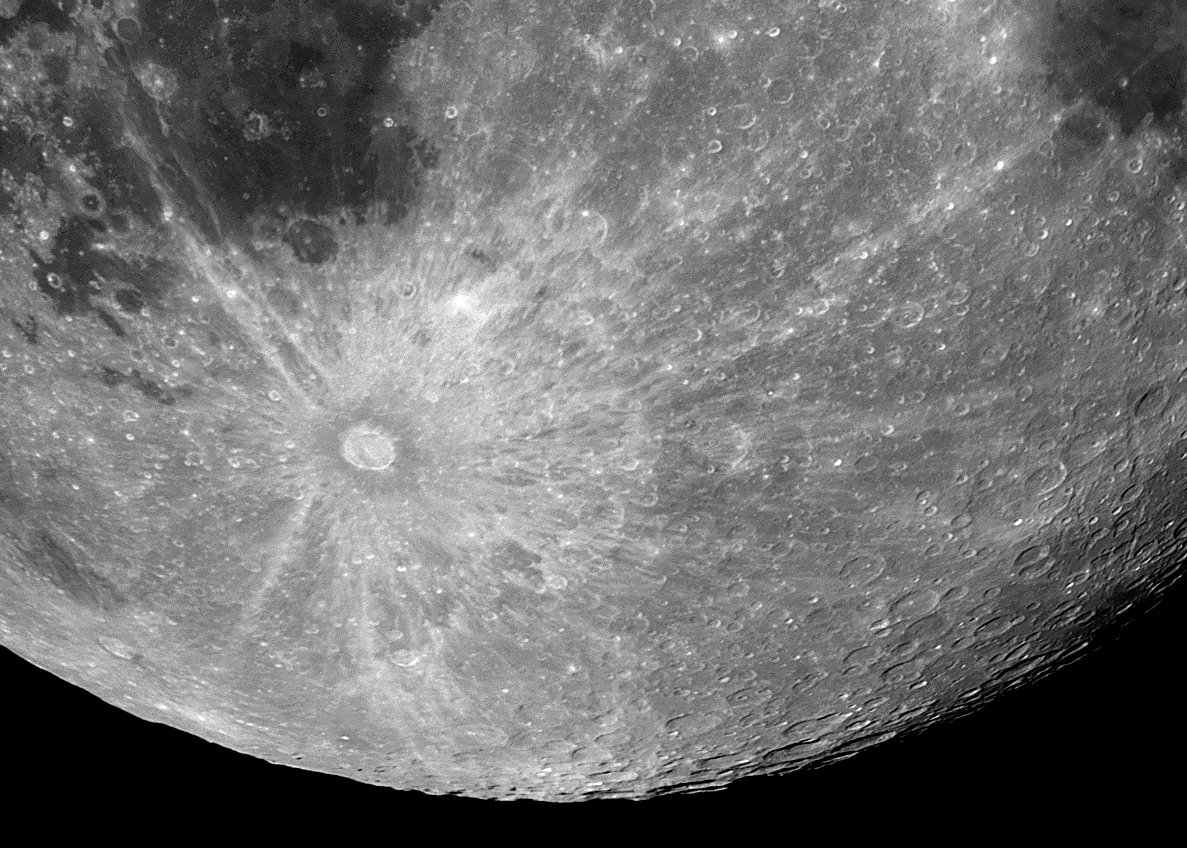
\includegraphics[width=0.9\textwidth]{Tycho_Full_Barrett.jpg}};
			\end{tikzpicture}
		\end{center}
	\end{columns}
\end{frame}

\begin{frame}{Copernicus}
	\begin{columns}
		\column{0.5\textwidth}
		\begin{center}
			\begin{tikzpicture}[scale=0.78]
				\node<1-2> {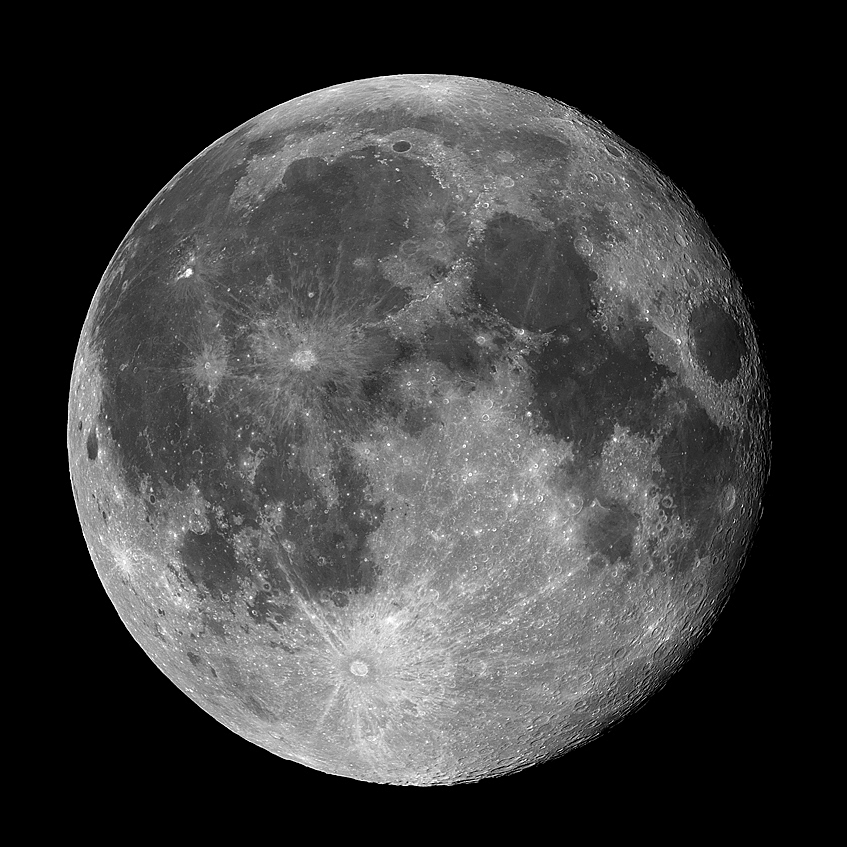
\includegraphics[width=0.9\textwidth]{FullMoon_Barrett.jpg}};
				\draw<2>[very thick, red] (-.9,.5) circle (4mm);
			\end{tikzpicture}
		\end{center}
		
		\column{0.5\textwidth}
		\begin{itemize}
			\item Named after Nicolaus Copernicus
			\item Large crater to West and in center of many darker seas
			\item Also has rays but they are more wandering
		\end{itemize}
		
	\end{columns}
\end{frame}

\begin{frame}{Sea of Tranquility}
	\begin{columns}
		\column{0.5\textwidth}
		\begin{itemize}
			\item Lower of the two seas to the East
			\item Lowlands expose darker rock, giving the distinct shade
			\item Apollo 11 landing was near the Southwest edge
		\end{itemize}
		\column{0.5\textwidth}
		\begin{center}
			\begin{tikzpicture}[scale=0.78]
				\node<1-3> {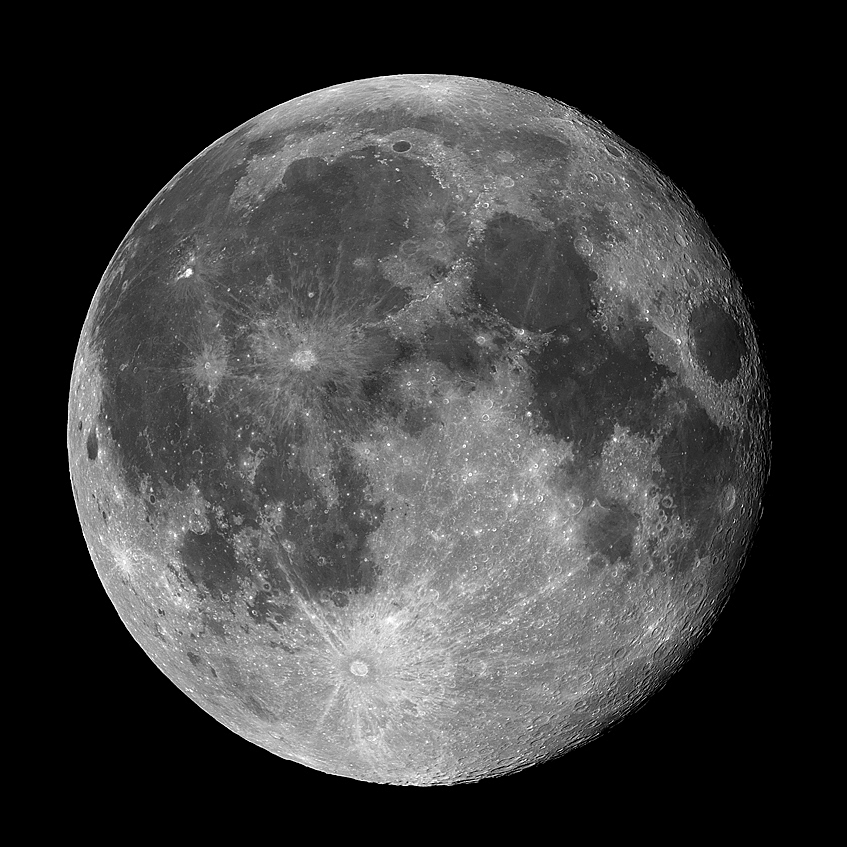
\includegraphics[width=0.9\textwidth]{FullMoon_Barrett.jpg}};
				\draw<2>[very thick, red] (1.2,0.2) circle (8mm);
				\draw<3>[very thick, orange] (1.1,-0.1) circle (2mm);
			\end{tikzpicture}
		\end{center}
	\end{columns}
\end{frame}

\renewcommand{\secimg}{SecPlanets.png}
\section{Planets}

\begin{frame}{Jupiter}
	\begin{columns}
		\column{0.5\textwidth}
		\begin{center}
			\begin{tikzpicture}
				\node<1> {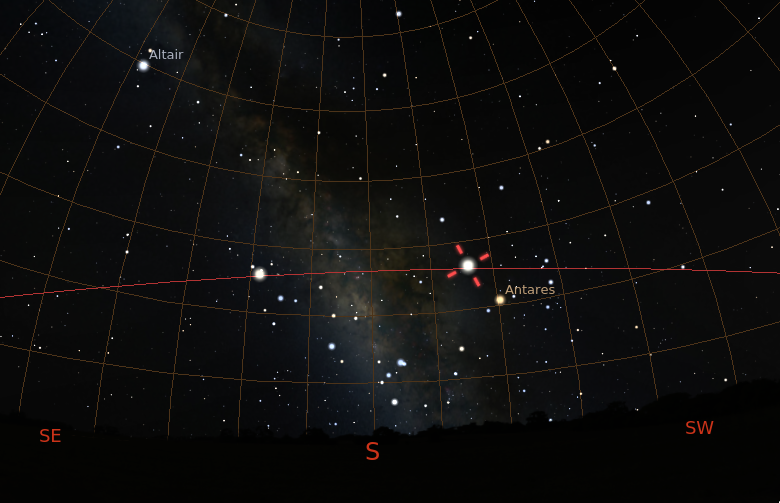
\includegraphics[width=\textwidth]{JupiterPosition.png}};
				\node<2> {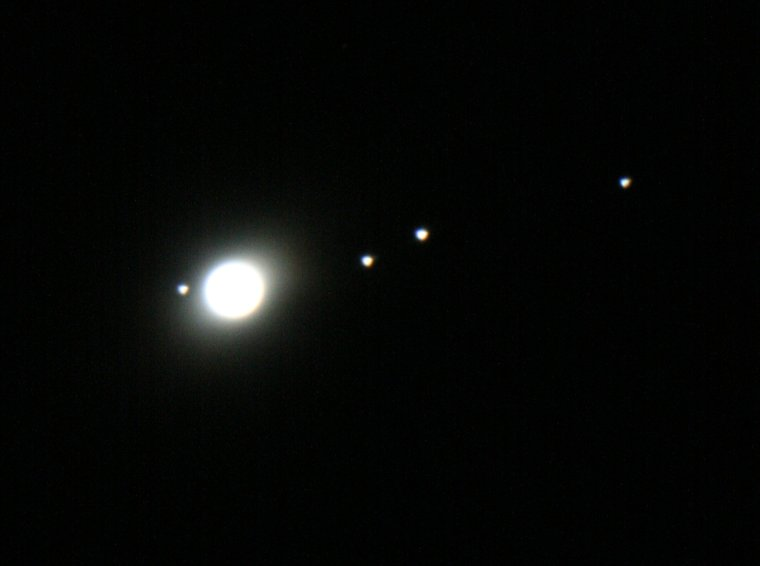
\includegraphics[width=\textwidth]{JupiterMoons.jpg}};
			\end{tikzpicture}
		\end{center}
		
		\column{0.55\textwidth}
		\begin{itemize}
			\item Largest of the planets. Will appear as a very large bright star in the sky.
			\item Look towards the South between 15 and 30 degrees above the horizon.
			\item If you see two really bright stars, Jupiter is the brighter and is the rightmost one at the moment.
			\item 4 moons easily visible with just binoculars
				\begin{itemize}
					\item Io, Europa, Ganymede and Callisto
					\item Sometimes 1 or 2 may be in front or behind the planet
				\end{itemize}
		\end{itemize}
	\end{columns}
\end{frame}

\begin{frame}{Saturn}
	\begin{columns}
		\column{0.5\textwidth}
		\begin{itemize}
			\item Also appears as a bright star in the sky.
			\item Currently near Jupiter but is the more leftmost bright point.
			\item Will just appear oblong in binoculars, really need a \alert{small telescope} to see the rings.
			\item Can sometimes see its largest moon Titan nearby.
		\end{itemize}
		\column{0.5\textwidth}
		\begin{center}
			\begin{tikzpicture}
				\node<1> {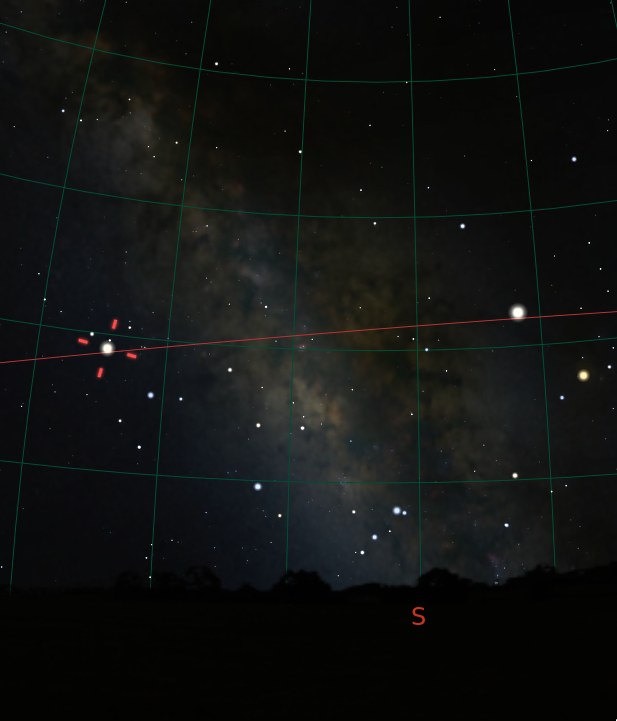
\includegraphics[width=\textwidth]{SaturnPosition.png}};
				\node<2> {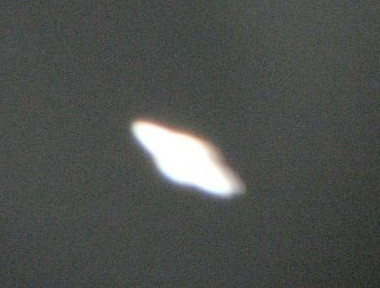
\includegraphics[width=\textwidth]{Saturn-through-binoculars.jpg}};
			\end{tikzpicture}
		\end{center}
		
	\end{columns}
\end{frame}

\begin{frame}{Venus and Mars}
	\begin{columns}
		\column{0.4\textwidth}
		\begin{center}
			\begin{tikzpicture}
				\node<1> {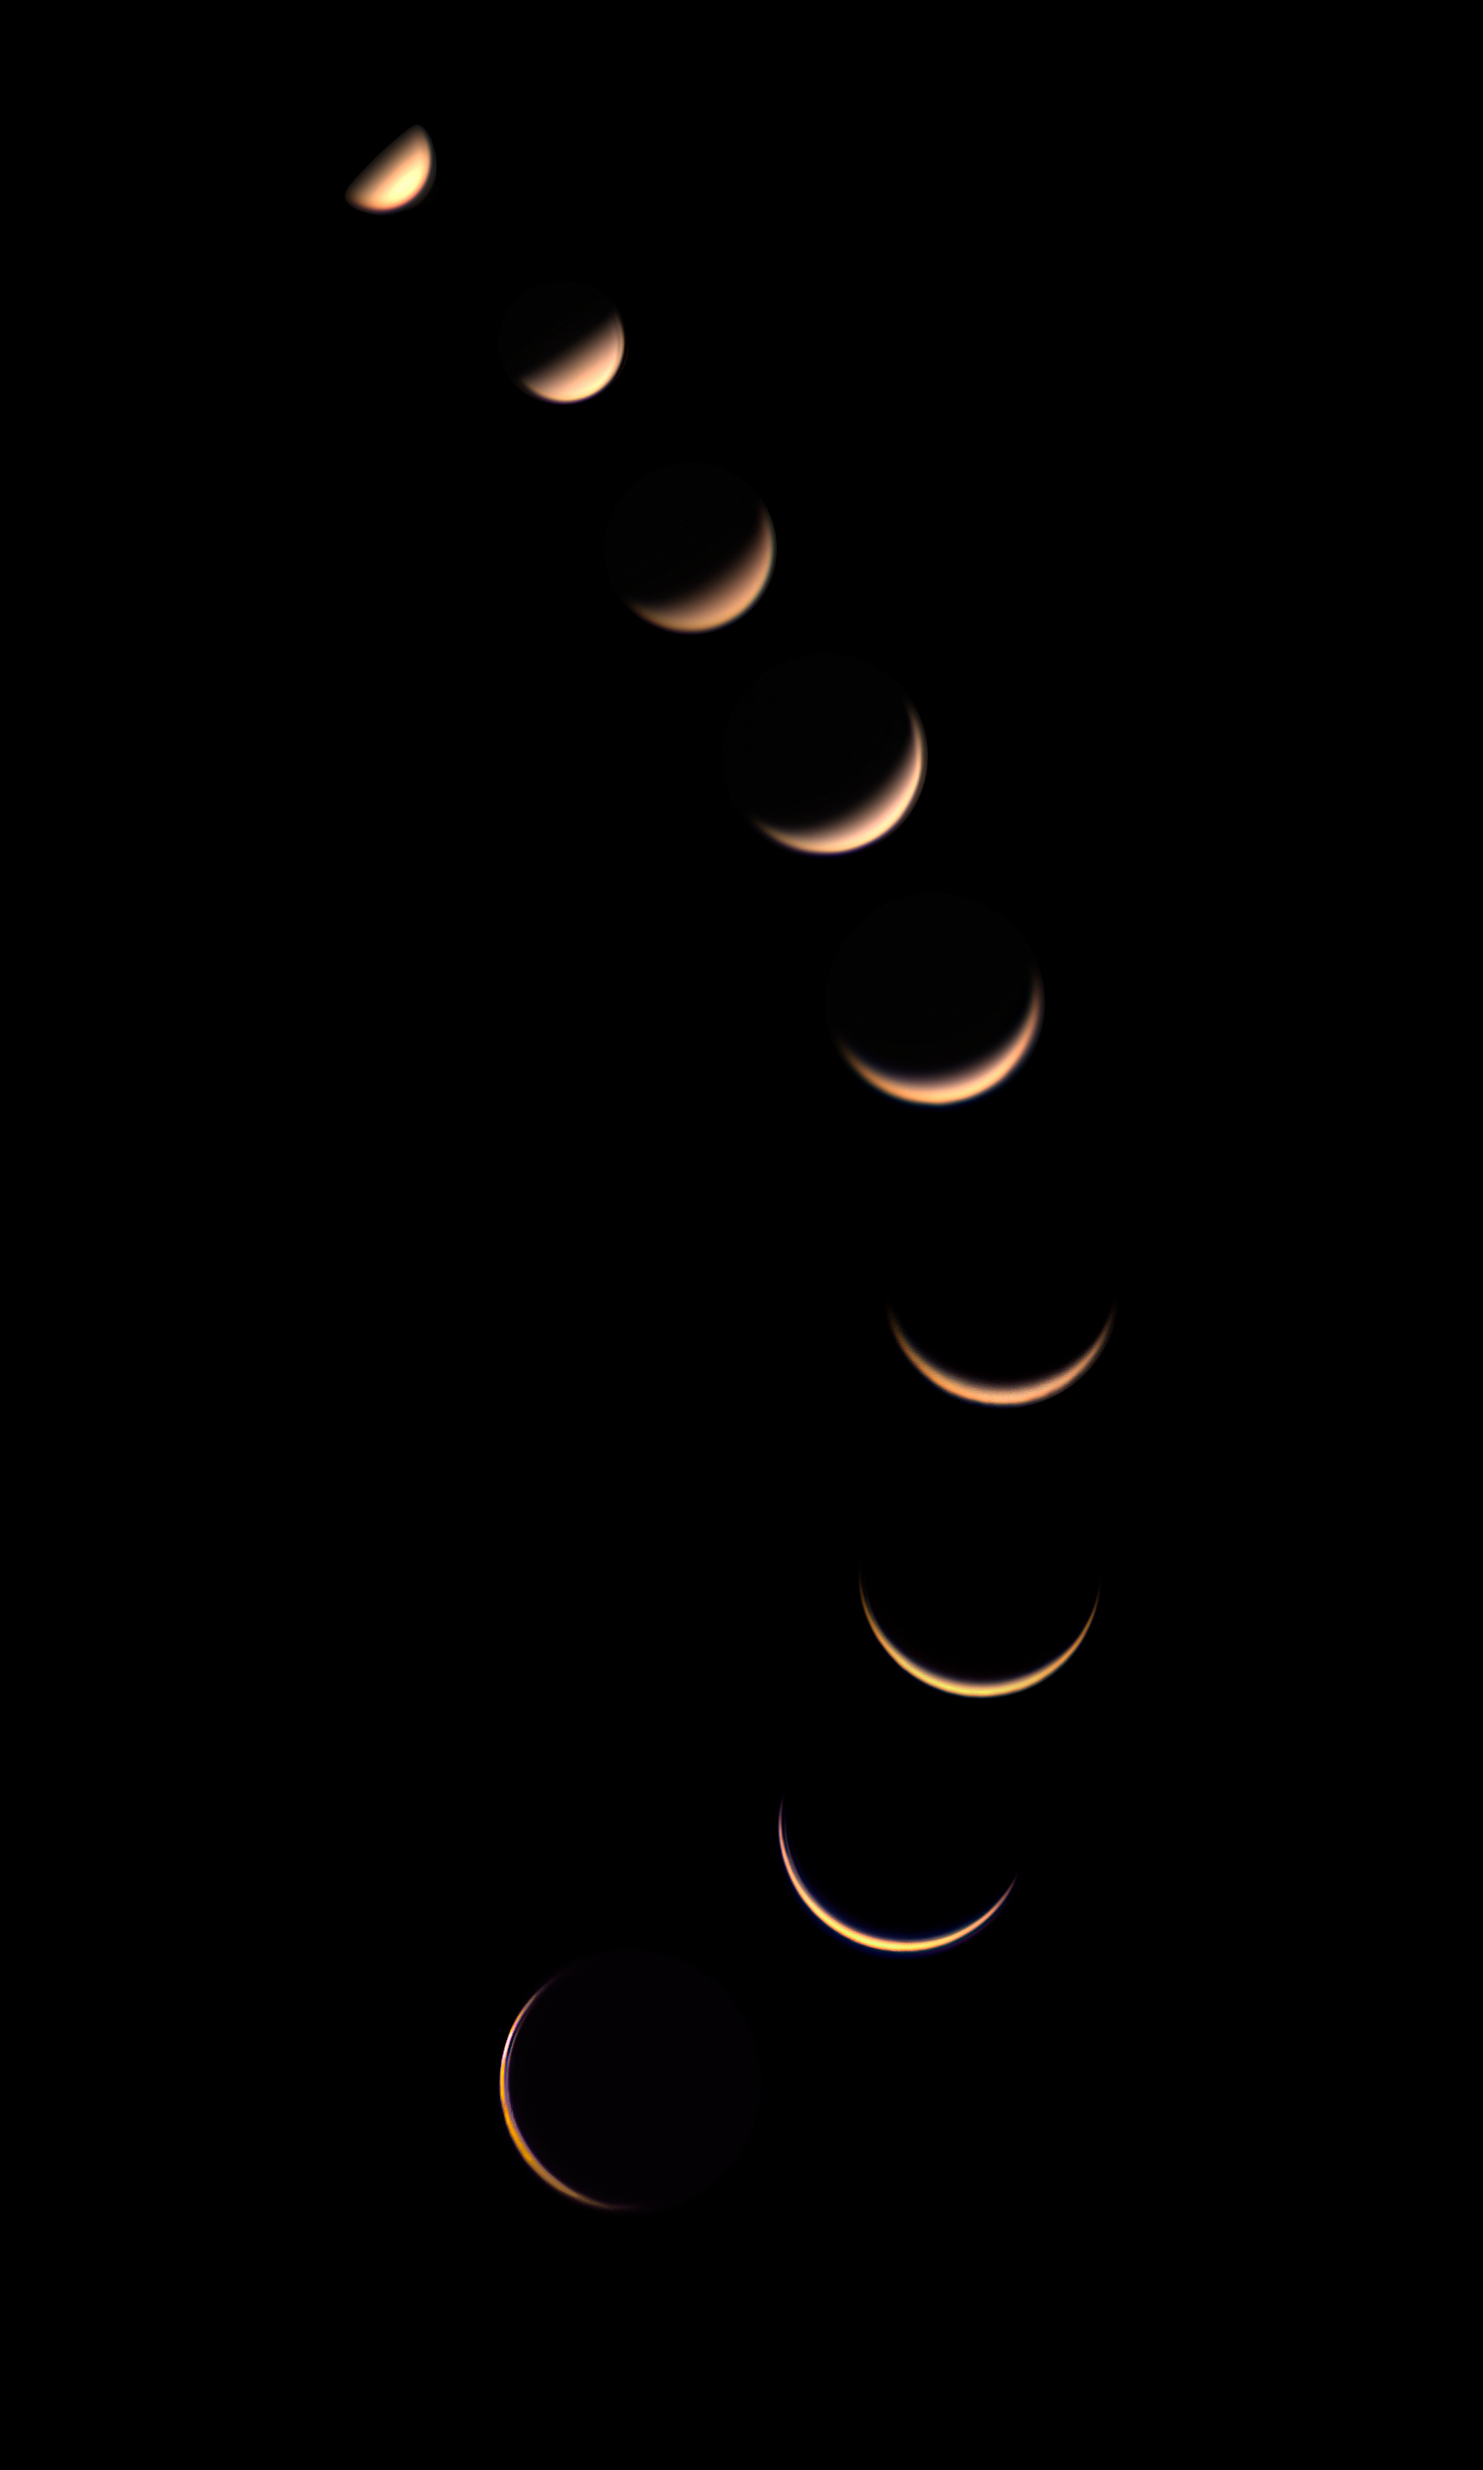
\includegraphics[width=.9\textwidth]{VenusPhases.jpg}};
				\node<2> {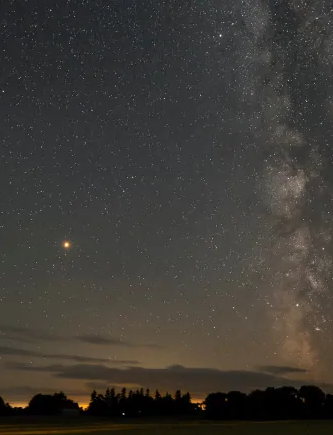
\includegraphics[width=\textwidth]{mars-opposition.png}};
			\end{tikzpicture}
		\end{center}
		\column{0.6\textwidth}
		\begin{itemize}
			\item<1-> Venus
				\begin{itemize}
					\item Brightest planet besides Jupiter
					\item Will always be hanging out near the Sun, so visible only in early evening or morning
						\begin{itemize}
							\item Currently so close to the Sun as to be invisible
						\end{itemize}
					\item Goes through visible phases and size changes
				\end{itemize}
			\item<2-> Mars
				\begin{itemize}
					\item Exhibits a reddish tinge
					\item Lies on the same ecliptic, so visible mainly looking South
					\item With telescope can sometimes make out polar caps
				\end{itemize}
		\end{itemize}
	\end{columns}
\end{frame}

\renewcommand{\secimg}{SecDeepSky.png}
\section{Deep Sky}

\begin{frame}{Deep Sky Basics}
	\begin{itemize}
		\item I will relate everything to 3 bright, easy, constellations. So you just need to be able to find them.
			\begin{itemize}
				\item Cassiopeia
				\item Orion
				\item The Big Dipper
			\end{itemize}
		\item Peripheral vision is more sensitive to light
			\begin{itemize}
				\item Don't stare directly at the dim object you are trying to see!
			\end{itemize}
		\item These all can be see in light-polluted areas, but it may be easier to find them the first time from a good dark location.
			
			
	\end{itemize}
	
\end{frame}

\begin{frame}{The Pleides: An Open Star Cluster}
	\begin{columns}
		\column{0.5\textwidth}
		\begin{center}
			\vspace{-8mm}
			\begin{tikzpicture}
				\node<1> {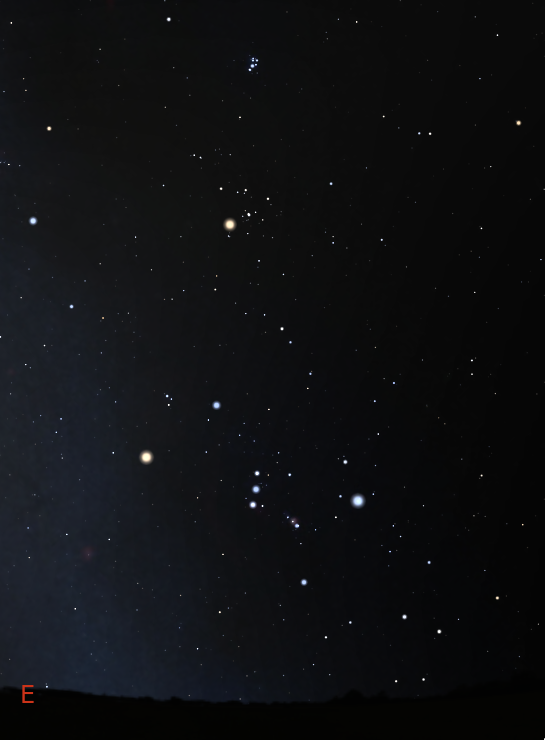
\includegraphics[width=\textwidth]{FindingPleides.png}};
				\node<2> {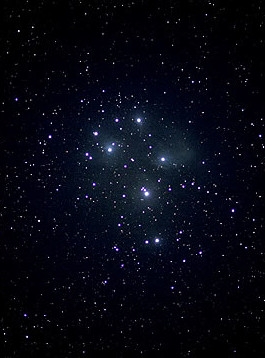
\includegraphics[width=\textwidth]{Pleides.jpg}};
			\end{tikzpicture}
		\end{center}
		\column{0.5\textwidth}
		\begin{itemize}
			\item Located in the constellation Taurus
				\begin{itemize}
					\item Can find by following the line of Orion's belt
					\item Or rapidly scan the sky looking for a blurry spot
				\end{itemize}
			\item Tightly packed bunch of young, bright blue stars
			\item Inspired the Subaru logo
		\end{itemize}
	\end{columns}
\end{frame}


\begin{frame}{Orion Nebula}
	\begin{columns}
		\column{0.5\textwidth}
		\begin{itemize}
			\item Brightest nebula to look at in the Northern hemisphere
			\item Resides in the ``dagger'' on Orion's belt
			\item Orion currently rises just before the Sun, but will be up earlier and earlier as we move toward winter.
		\end{itemize}
		\column{0.5\textwidth}
		\begin{center}
			\begin{tikzpicture}
				\node<1> {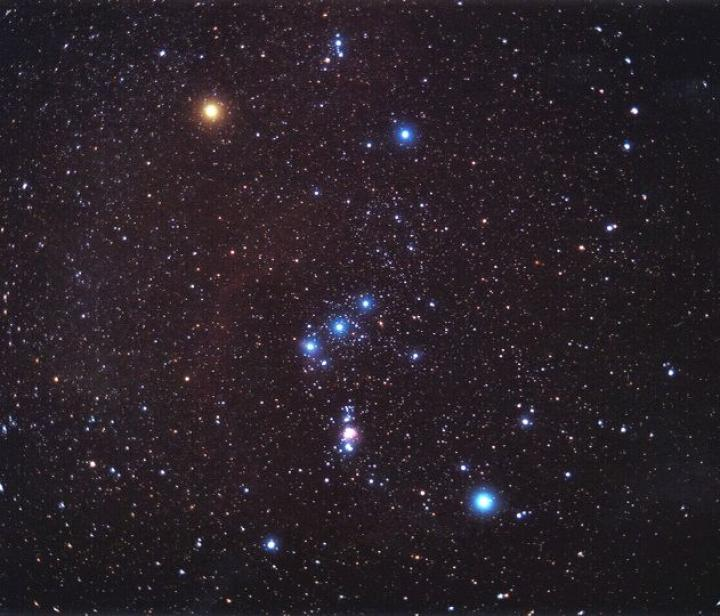
\includegraphics[width=\textwidth]{orion_constellation.jpg}};
				\node<2> {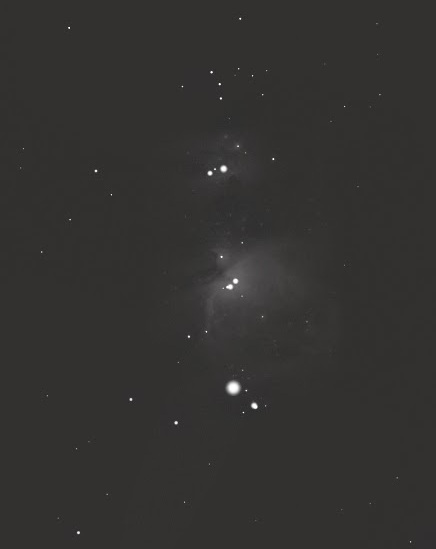
\includegraphics[width=\textwidth]{OrionNebula_Binocs.jpg}};
			\end{tikzpicture}
		\end{center}
	\end{columns}
\end{frame}

\begin{frame}{Andromeda Galaxy}
	\begin{columns}
		\column{0.5\textwidth}
		\begin{itemize}
			\item Our nearest galactic neighbor!
			\item Definitely easier to spot away from light pollution
			\item Follow a trail of constellations to help find it:
				\begin{itemize}
					\item Cassiopeia (the ``W'')
					\item Pegasus (a big square)
					\item Andromeda (two ``legs'' attached to the square)
				\end{itemize}
			\item Will appear an oblong fuzzy blob with naked eyes, much more detail visible with binoculars
		\end{itemize}
		
		\column{0.5\textwidth}
		\begin{center}
			\vspace{-5mm}
			\begin{tikzpicture}[
				star/.style={circle, minimum size=1mm, inner sep=0pt,},
				scale=0.78
				]
				\node {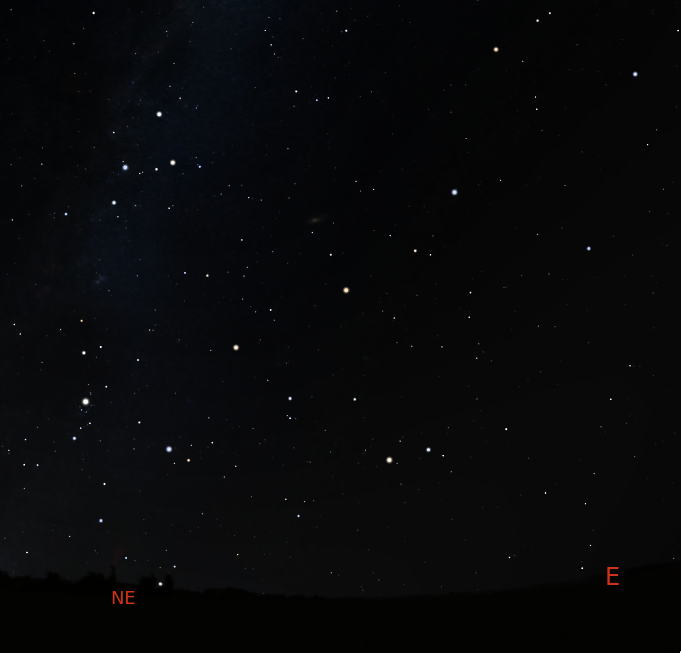
\includegraphics[width=\textwidth]{Cass_n_Peg.png}};
				\node[star] (c1) at (-2.82,1.15) {};
				\node[star] (c2) at ($(c1)+(.5,.12)$) {};
				\node[star] (c3) at ($(c2)+(.11,.37)$) {};
				\node[star] (c4) at ($(c3)+(.48,.06)$) {};
				\node[star] (c5) at ($(c4)+(-.14,.48)$) {};

				\node[star] (p1) at (1.18,1.37) {};
				\node[star] (p2) at ($(p1)+(.43,1.47)$) {};
				\node[star] (p3) at ($(p2)+(1.43,-.26)$) {};
				\node[star] (p4) at ($(p3)+(-.48,-1.78)$) {};

				\node[star] (a1) at ($(p1)+(-.41,-.59)$) {};
				\node[star] (a2) at ($(a1)+(-.71,-.4)$) {};
				\node[star] (a3) at ($(a2)+(-1.14,-.6)$) {};
				\node[star] (a4) at ($(p1)+(-.66,-.44)$) {};
				\node[star] (a5) at ($(a4)+(-.62,-.20)$) {};
				\node[star] (a6) at ($(a5)+(-1.5,-.20)$) {};

				\draw<2->[red, thick] (c1) -- (c2) -- (c3) -- (c4) -- (c5);
				\draw<3->[orange, thick] (p1) -- (p2) -- (p3) -- (p4) -- (p1);
				\draw<4->[cyan,thick] (p1) -- (a1) -- (a2) -- (a3) (p1) -- (a4) -- (a5) -- (a6);
				\draw<5->[green,-latex, thick] (a2) -- ($(a2)!1.9!(a5)$);
			\end{tikzpicture}
		\end{center}
	\end{columns}
\end{frame}

\begin{frame}{Andromeda thru Binoculars}
	\begin{center}
		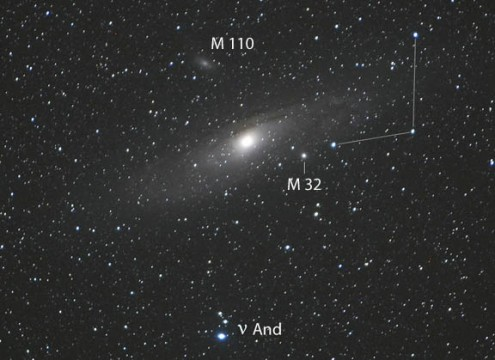
\includegraphics[width=0.8\textwidth]{AndromedaGalaxy.jpg}
	\end{center}
\end{frame}

\begin{frame}{Hercules Cluster: A Globular Cluster}
	\begin{columns}
		\column{0.45\textwidth}
		\begin{itemize}
			\item Located in constellation Hercules
				\begin{itemize}
					\item Rests between the bright stars Vega and Arcturus
					\item The handle of the big dipper points towards Arcturus (roughly)
				\end{itemize}
			\item Incredibly dense regions of old, yellow/golden stars
			\item Generally live above or below the disk of the Milky Way
		\end{itemize}
		
		\column{0.55\textwidth}
		\begin{center}
			\begin{tikzpicture}[
				star/.style={circle, minimum size=1mm, inner sep=0pt,},
				scale=0.78
				]
				\node<1-5> {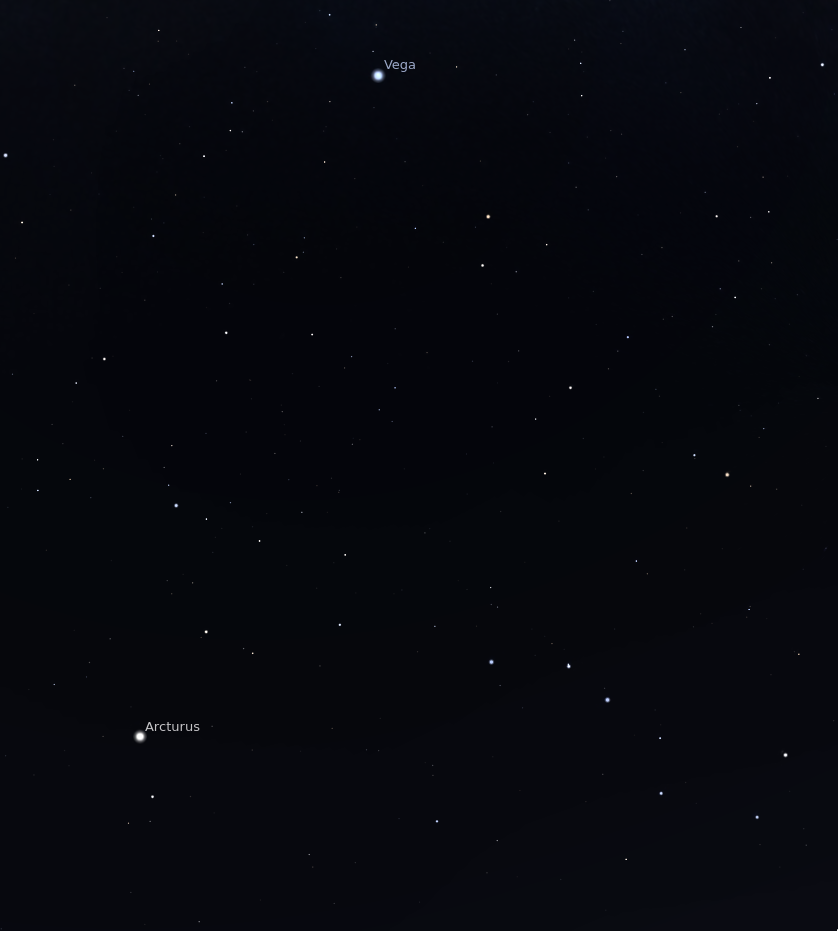
\includegraphics[width=\textwidth]{FindingHercules.png}};
				\node[star] (bd1) at (3.34,-2.65) {};
				\node[star] (bd2) at ($(bd1)+(245:.6)$) {};
				\node[star] (bd3) at ($(bd2)+(167:.9)$) {};
				\node[star] (bd4) at ($(bd3)+(92:.5)$) {};
				\node[star] (bd5) at ($(bd4)+(142:.6)$) {};
				\node[star] (bd6) at ($(bd5)+(138:.48)$) {};
				\node[star] (bd7) at ($(bd6)+(178:.72)$) {};

				\node[star] (arc) at (-2.52,-2.48) {};
				\node[star] (veg) at (-.36,3.55) {};

				\node[star] (h1) at (-1.1,1.9) {};
				\node[star] (h2) at ($(h1)+(280:.7)$) {};
				\node[star] (h3) at ($(h2)+(180:.8)$) {};
				\node[star] (h4) at ($(h3)+(90:.45)$) {};

				\draw<2-5>[red, thick] (bd1)--(bd2)--(bd3)--(bd4)--(bd1) (bd4)--(bd5)--(bd6)--(bd7);
				\draw<3-5>[cyan, thick, dashed] (arc) -- (veg);
				\draw<4-5>[orange, thick] (h1)--(h2)-- coordinate[pos=.3](clu)(h3)--(h4)--(h1);
				\draw<5-5>[green, thick, latex-] (clu) -- +(-40:.5);
				\node<6> {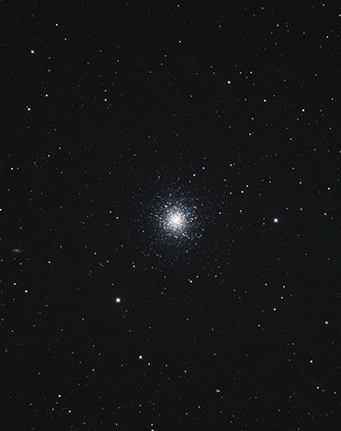
\includegraphics[width=.9\textwidth]{HerculesCluster.png}};
			\end{tikzpicture}
		\end{center}
	\end{columns}
\end{frame}

\begin{frame}{Perseid Meteor Shower}
	\begin{columns}
		\column{0.5\textwidth}
		\begin{center}
			\vspace{-5mm}
			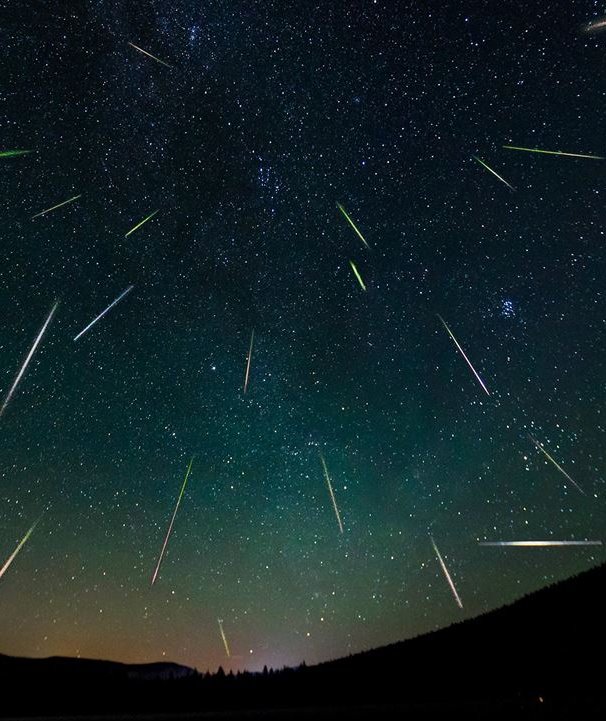
\includegraphics[width=1.1\textwidth]{Perseids.png}
		\end{center}
		
		\column{0.5\textwidth}
		\begin{itemize}
			\item Caused by debris from Comet Swift-Tuttle burning up in the atmosphere
			\item \alert{Radiant} will appear to be in the constellation Perseus, just below Cassiopeia
				\begin{itemize}
					\item In truth though, just look up. You'll see them everywhere!
				\end{itemize}
				
			\item Peak mornings are August 11,12,13
				\begin{itemize}
					\item But watch starting now! A large moon will obscure viewing on those days
				\end{itemize}
		\end{itemize}
	\end{columns}
\end{frame}

\begin{frame}{Notable Satellites}
	\begin{columns}
		\column{0.5\textwidth}
		\begin{itemize}
			\item The International Space Station (ISS)
				\begin{itemize}
					\item Semi-reliable in when it passes overhead
					\item Appears as a quickly moving, very bright star
				\end{itemize}
			\item Iridium Flares
				\begin{itemize}
					\item From Iridium communication satellites
					\item Appear as a really slow, really bright shooting star
				\end{itemize}
			\item Can get info or alerts about upcoming passes from Heavens-Above website or app
		\end{itemize}
		
		\column{0.5\textwidth}
		\begin{center}
			\inlineMovie{../Vids/ISS.ogv}{../Vids/ISS.png}{width=\textwidth}
			\inlineMovie{../Vids/Flare.ogv}{../Vids/Flare.png}{width=\textwidth}
		\end{center}
	\end{columns}
\end{frame}

\begin{frame}{Wrap Up}
	\begin{itemize}
		\item Even in cloudy and light-polluted Salem there are fun things to check out in the sky!
			\begin{itemize}
				\item Lunar details
				\item Nearby planets
				\item Bright deep sky objects
				\item Debris in or just above our atmosphere
			\end{itemize}
		\item Finding said objects is not rocket science
		\item Even simple binoculars can take your observing night to the next level!
	\end{itemize}
\end{frame}

\begin{frame}{Some Resources}
	\begin{itemize}
		\item Stellarium: Free planetarium software
		\item \url{www.heavens-above.com}: Satellite predictions
		\item Sky Map: Android app showing location of objects in sky
	\end{itemize}
	\vspace{5mm}
	\begin{itemize}
		\item Photo credits:
			\begin{itemize}
				\item Frank Barrett for images of the Moon
				\item \url{www.bestbinocularreviews.com} for image of Saturn
				\item Max Mallon for phases of Venus
				\item Malcolm Park for image of Mars
				\item Bob King for image of Andromeda
			\end{itemize}
			
	\end{itemize}
	
	
\end{frame}








\end{document}

